\section{BCD to Binary conversion}
\subsection{Aim}
To convert BCD to Binary

\subsection{Code}
\begin{lstlisting}
DATA SEGMENT
    BCD DB 29H
    BIN DB ?
DATA ENDS

CODE SEGMENT
ASSUME CS:CODE, DS:DATA
START:
    MOV AX, DATA                   
    MOV DS, AX
    MOV AH, BCD
    MOV BH, AH
    AND BH, 0FH
    AND AH, 0F0H
    ROR AH, 04
    MOV CL, 10
    MOV AL, AH
    AND AX, 00FFH
    MUL CL
    ADD AL, BH
    MOV BIN, AL
    MOV AH, 04CH
    INT 21H
CODE ENDS
END START
\end{lstlisting}

\subsection{Output}
\begin{center}
	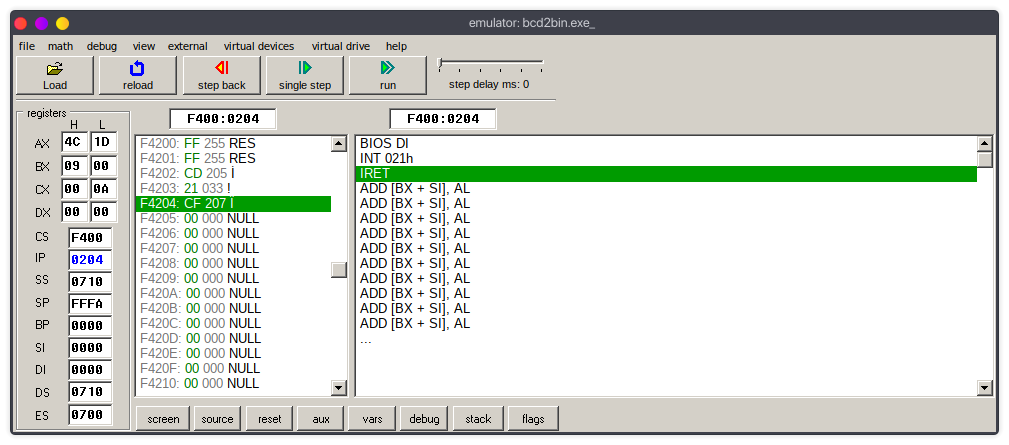
\includegraphics[width=0.90\textwidth]{img/p13/ss1.png}
	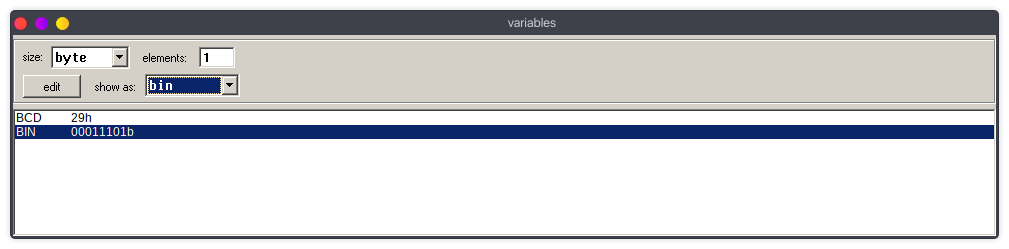
\includegraphics[width=0.90\textwidth]{img/p13/ss2.png}
\end{center}

\subsection{Result}
A BCD number was converted to decimal